% begin module function-rep
\begin{frame}[t]
\frametitle{Representations of Functions}
There are four ways to represent a function:
\begin{enumerate}
\item<handout| 2-| alert@2>  Algebraically (by a formula).
\item<handout| 3-| alert@3>  Numerically (by a table of values).
\item<handout| 4-| alert@4>  Verbally (by a description in words).
\item<handout| 5-| alert@5>  Visually (by a graph).
\end{enumerate}

\only<handout:0| 2>{
\begin{example}[The Area of a Circle]
The area $A$ of a circle depends on its radius $r$.  The rule that connects $r$ and $A$ is given by the equation $A = \pi r^2$.  
\end{example}
}
\only<handout:0| 3>{
\begin{example}[The Human Population of the World]
\begin{columns}
\column{.7\textwidth}
The human population of the world $P$ depends on the time $t$.  The table on the right gives estimates of the world population $P(t)$ at time $t$, for certain years.  For example,
\[
P(2010) \approx 6,797,000,000 .
\]
\column{.3\textwidth}
\begin{tabular}{|c|c|}
\hline
 & Population \\
Year & (millions) \\
\hline
%1900 & 1650 \\
%1910 & 1750 \\
%1920 & 1860 \\
%1930 & 2070 \\
%1940 & 2300 \\
%1950 & 2560 \\
1960 & 3040 \\
1970 & 3710 \\
1980 & 4450 \\
1990 & 5280 \\
2000 & 6080 \\
2010 & 6797 \\
\hline
\end{tabular}
\end{columns}
\end{example}
}
\only<handout:0| 4>{
\begin{example}[The Cost of Mailing a Letter]
The cost $C$ of mailing a first-class letter depends on the weight $w$ of the letter.  Although there is no simple formula that connects $w$ and $C$, the post office has a rule for determining $C$ when $w$ is known.
\end{example}
}
\only<handout:0| 5>{
\begin{example}[ECG Readings]
The electrical activity of the heart, as recorded by an electrocardiograph machine, is a function of the elapsed time $t$.  The graph below depicts the ECG data recorded for a patient at a hospital.

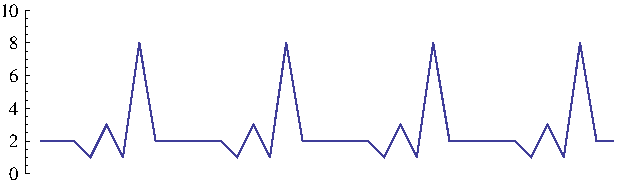
\includegraphics[height=2.5cm]{precalculus/pictures/01-01-ECG.pdf}

\end{example}
}
\end{frame}


\begin{frame}
\frametitle{The Definition of a Function}

\begin{definition}[Function]
A function $f$ is a rule that assigns to each element $x$ in a set $D$ exactly one element, called $f(x)$, in a set $E$.
\end{definition}

\uncover<2->{
\begin{definition}[Domain and Range]
The set $D$ is called the domain and $E$ is called the range.  We consider functions for which the domain and range are sets of real numbers.
\end{definition}
}

\uncover<3->{
\begin{definition}[Value of $f$ at $x$]
The number $f(x)$ is called the value of $f$ at $x$, and is read ``$f$ of $x$.''
\end{definition}
}

\uncover<4->{
\begin{definition}[Independent and Dependent Variables]
A symbol that represents an arbitrary number in the domain is called an independent variable.  A symbol that represents an arbitrary number in the range is called a dependent variable.
\end{definition}
}
\end{frame}
% end module function-rep
